\documentclass[10pt,twocolumn]{article}

\usepackage[letterpaper,margin=0.72in,columnsep=0.25in]{geometry}
\usepackage[T1]{fontenc}
\usepackage[utf8]{inputenc}
\usepackage{lmodern}
\usepackage{microtype}
\usepackage{amsmath,amssymb}
\usepackage{booktabs}
\usepackage{graphicx}
\usepackage[hidelinks]{hyperref}
\usepackage{xurl}
\usepackage{enumitem}
\usepackage{caption}
\usepackage[round,authoryear]{natbib}
\usepackage{flushend}

\setlist{nosep,leftmargin=*}
\captionsetup{font=small,labelfont=bf}
\newcommand{\Description}[1]{}

\hypersetup{
  pdftitle={LLMs Read the Room Better Than Humans: Comparative Social-Transmission Prediction by LLMs and Human Judges},
  pdfauthor={Victor Lavrenko},
  pdfsubject={Large language model capabilities, audience preference prediction, generation and self-evaluation},
  pdfkeywords={large language models, audience modeling, preference prediction, self-evaluation, generation, social transmission}
}

\title{\textbf{LLMs Read the Room Better Than Humans}\\\large Comparative Social-Transmission Prediction by LLMs and Human Judges}
\author{Victor Lavrenko\\
\small PeaceTech VC, Jerusalem, Israel\\
\small \texttt{victor@peacetech.vc}}
\date{17 September 2026}

\begin{document}
\raggedbottom
\clubpenalties 4 10000 10000 8000 0
\widowpenalties 4 10000 10000 8000 0
\displaywidowpenalty=10000
\emergencystretch=1.2em
\setlength{\textfloatsep}{7pt plus 2pt minus 2pt}
\setlength{\floatsep}{6pt plus 2pt minus 2pt}
\setlength{\intextsep}{6pt plus 2pt minus 2pt}
\maketitle

\begin{abstract}
LLMs are notorious for producing generic, formulaic ``AI slop.'' Yet the same models may already know surprisingly well what kinds of narratives people appreciate; the failure may be in turning that knowledge into generation. We probe this hidden audience model through social transmission: given two human-written posts, can an LLM predict which one people chose to retransmit? Sharing is a stronger behavioral commitment than merely liking or rating a message, making it a useful revealed-preference signal. On 1,142 same-author/same-link Twitter pairs, Gemini reaches 79.7\% versus historical human references of 61.3\% for individuals and 73.0\% for majority judgment. In 70 blind contemporary sessions, Gemini scores 77.7\% versus 54.1\% for matched human choices. Prompt/order perturbations preserve the frontier result, confidence isolates 92--96\% top-quartile subsets, and fresh 2026 Bluesky outcomes reproduce the signal. A practical text-only ceiling near 85\% suggests that frontier LLMs already capture much of the audience-response signal available from text, motivating evaluation-guided generation.
\end{abstract}

\noindent\textbf{Keywords:} large language models; social transmission; comparative prediction; audience modeling; uncertainty; robustness; inference-time evaluation.
\vspace{0.7em}

\section{Introduction}
LLMs have a visible writing problem: even very capable systems routinely produce generic, formulaic, over-polished prose---the style now commonly dismissed as ``AI slop.'' The obvious explanation is that models do not understand what people actually appreciate. This paper tests a more interesting possibility: strong LLMs may already contain a remarkably good model of human narrative preference, but fail to use that knowledge reliably when generating their own text.

We probe that latent knowledge without asking the model to write. Instead, humans and LLMs judge the same alternatives written by other humans: which framing did people value enough to pass on? We operationalize this as \emph{comparative social-transmission prediction}. Retransmission is useful because it is revealed behavior, not a survey rating, and because sharing a message with one's own audience entails a stronger behavioral commitment than simply clicking Like. If an LLM can reliably predict what people retransmit, it has learned something consequential about which narratives work for human audiences even if its default prose does not consistently express that knowledge.

The setting comes from the topic- and author-controlled natural experiment of \citet{tan2014}: two posts from the same account point to the same URL but use different wording or framing. Their human study reported 61.3\% average individual accuracy and 73.0\% majority-vote accuracy over 39 judgments per pair; their supervised classifier reached 65.6\% on held-out TAC data. On the 1,142-pair HypoBench hydration of the task, the six contemporary LLMs evaluated here reach 63.5--79.7\%.

We add a direct contemporary human comparison. In the public \href{https://beat-the-robot.peacetech.vc/}{\emph{Beat the Robot}} deployment, 70 completed first-round sessions yielded 1,400 blind choices before feedback. Fixed-model comparisons on the same items show positive model--human gaps for all six model families; Gemini reaches 77.7\% versus 54.1\% for matched recorded choices, a +23.6-point gap with a crossed session/item bootstrap interval of +17.6 to +29.4 points.

We also test whether the frontier result survives changes in elicitation and data source. On a deterministic 100-pair subset, three strong/provider-diverse models remain accurate under equivalent prompt wording and X/Y reversal, and explicit confidence sharply ranks prediction quality: the most-confident quartile reaches 92--96\% accuracy. A fresh August 2026 Bluesky replication shows similar signal on newly collected same-author/same-destination outcomes.

Finally, we argue that 100\% is the wrong practical denominator for text-only prediction of a stochastic social outcome. Timing, exposure, follower state, competing events, and cascade realization can affect which message wins even when the texts are fixed. A data-anchored sensitivity model places the practical text-only ceiling near 85\%, with an 82--90\% envelope. Under that scale, the strongest model captures a large fraction of the improvement available from chance to the text-only target.

We address five research questions: \textbf{RQ1} benchmarks current LLMs against historical human and machine baselines; \textbf{RQ2} tests matched contemporary human judgments; \textbf{RQ3} tests whether model confidence identifies more reliable predictions; \textbf{RQ4} tests prompt wording and X/Y reversal; and \textbf{RQ5} tests replication on fresh Bluesky outcomes.

Our contribution is a capability map: a six-model historical comparison, matched contemporary human judgments, crossed-cluster uncertainty, confidence/selective-prediction analysis, prompt/order robustness, and a fresh-platform replication. Together they show that current LLMs can predict aggregate social transmission substantially better than the human judgments available in these datasets.

\section{Related Work}
\subsection{Social transmission as revealed narrative preference}
Sharing is not identical to liking or semantic understanding. Transmission can reflect practical value, emotional arousal, identity signaling, novelty, social utility, and communication motive \citep{berger2012,berger2025}. Raw engagement also depends on author reach, topic, time, media, network position, and cascade dynamics.

\citet{tan2014} reduce several of these sources of variance with topic- and author-controlled (TAC) pairs: the same account posts different messages about the same URL, and the task is to predict which propagates further. Across 106 subjects, average subject accuracy was 61.3\%; each pair received 39 judgments, and majority voting reached 73.0\%. Their task-specific system reached 66.5\% in cross-validation and 65.6\% on held-out TAC data using linguistic features plus bag-of-words. The present work extends this line with substantially stronger general-purpose LLMs, matched contemporary human judgments, uncertainty and robustness analysis, and fresh-platform replication.

HypoBench \citep{liu2025hypo} later hydrated the TAC task into a machine-evaluable benchmark. Broader virality settings remain difficult: Reddit-V reports weak zero-shot LLM performance relative to task-specific multimodal systems in a less controlled setting \citep{elamrany2025}, while persona-prompted agents show modest prediction of individual social-media reactions in some settings \citep{bojic2026}. Our task is narrower: third-person comparative judgment with author and destination matched.

\subsection{LLMs as evaluators and uncertainty reporters}
LLMs can sometimes evaluate outputs or estimate their likelihood of correctness more reliably than they can produce a correct answer on the first attempt. \citet{kadavath2022} show useful self-knowledge and calibration under appropriate elicitation. Self-Refine uses post-hoc feedback for iterative revision \citep{madaan2023}, and Self-Rewarding Language Models use model judgments as preference signals during training \citep{yuan2024}. Intrinsic self-correction can also fail without reliable feedback \citep{huang2024}, making direct measurement of evaluator quality important.

Our setting isolates an external evaluation capability: choosing between human-authored alternatives according to realized audience behavior. This provides a measurable bridge between social prediction and evaluation-guided generation.

\subsection{A text-only target below 100\%}
Prediction of a realized social outcome differs from classification under a deterministic label rule. Even after author and destination are matched, timing, exposure, follower availability, competing events, network state, and cascade dynamics remain outside the text. The natural target is therefore the optimal decision rule conditioned on text alone. Section~\ref{sec:ceiling} models that target explicitly and relates the observed frontier to a practical 85\% text-only ceiling.

\section{Method}
\subsection{Historical Twitter benchmark and frozen model evaluation}
We use 1,142 historical pairs from the public HypoBench retweet split \citep{liu2025hypo}, which hydrates the TAC task introduced by \citet{tan2014}. Every item contains two tweets from the same account linking to the same URL and a binary label indicating which received more retweets.

Pair orientation was deterministically randomized independently of the gold label. Models saw only the two texts and the instruction to choose the higher-retweet message; no counts, timestamps, tools, or gold labels were supplied. The prompt additionally requested ``Close call: Yes/No.'' The frozen six-model panel is: \nolinkurl{google/gemini-3.7-flash}, \nolinkurl{openai/gpt-5.6-sol}, \nolinkurl{anthropic/claude-opus-4.8}, \nolinkurl{qwen/qwen3.7-max}, \nolinkurl{qwen/qwen3.7-flash}, and \nolinkurl{deepseek/deepseek-v4-flash-0731}. Frozen predictions, orientation, and close-call fields are pinned to the public \texttt{human-retweet-v4} snapshot at commit \texttt{972ad75d...f6fe}, SHA-256 \texttt{d656faca...825f}.

Historical human references come from Tan et al.'s 100-pair AMT experiment: 106 subjects overall, 39 judgments per pair, 61.3\% average subject accuracy, and 73.0\% majority-vote accuracy. Their task-specific supervised classifier reached 65.6\% on a held-out TAC set. Matched human--model inference uses the contemporary study below.

\subsection{Prompt, order, and confidence robustness}
We ran a fully automatic robustness experiment on a deterministic 100-pair subset of the historical benchmark. Pairs were ranked by SHA-256 of \texttt{20260917|pair\_id}; the first 100 were fixed before inference. We evaluated Gemini 3.7 Flash, GPT-5.6 Sol, and Claude Opus 4.8 through OpenRouter on 17 September 2026.

The prompt check uses the paper prompt and a concise semantically equivalent rephrasing. The order check reruns the paper prompt with X and Y swapped, then maps the response back to the underlying tweet identity; the primary statistic is canonical-choice consistency. The confidence check asks for X/Y plus an integer confidence from 50 to 100. Each condition uses a fresh chat context, no system prompt, no tools, temperature 0, and \texttt{max\_tokens=1200}. The runner permits two outer attempts, disables hidden SDK retries, archives prompts and raw responses, and uses explicit parsing rules. All prespecified outputs were valid.

\subsection{Blind contemporary web study}
We deployed the same binary task as the voluntary public game \emph{Beat the Robot}. The frozen export at 9 September 2026 04:32:50 UTC contains 99 started sessions and 70 completed primary Round-1 sessions, yielding 1,400 recorded choices. Recruitment was by convenience through public, personal, and academic-network sharing. A completed Round 1 contains 20 blind decisions made before correctness feedback or model scores were shown.

The public deployment required no login. Fifty-nine completions used protocol v4, ten v3, and one v1; the binary X/Y task remained the primary outcome. Sixty-nine of 70 completed sessions self-reported non-native English and one native English. Marketing experience was none in 46, learner/student in 10, and professional in 14; early-Twitter use was none in 44, occasional in 24, and regular in two.

The game displayed the highest-scoring fully answering model on each session's 20-item set as the ``featured robot.'' Scientific comparisons use each fixed model family separately. Five model families have complete predictions for 69 sessions; Qwen 3.7 Max has complete 20-item coverage for 62 sessions. Matched analysis uses only complete sessions for the model being evaluated. Round 1 is the primary analysis; later rounds had eight and two completions respectively.

\subsection{Human-subjects data handling and ethics}
Participation was voluntary and required explicit consent before the first trial. Players could use a nickname or play anonymously; no account login was required. Stored variables were trial choices, response times, and three coarse background questions. Public artifacts remove nicknames, original session identifiers, and exact timestamps. The study was conducted independently outside an institutional research program with an applicable review process, and no institutional review board reviewed it.

\subsection{Fresh August 2026 Bluesky replication}
The fresh-data component was collected from Bluesky activity in a frozen 84-hour window from 27--30 August 2026. The discovery crawl produced 35,946 eligible candidate rows from 3,175 authors with repeated-link candidates. A deterministic finalizer applied same-author/same-structured-destination, at-most-12-hour gap, materially different text, mature-outcome, and decisive-outcome rules: the winner required at least eight reposts, a margin of at least five, and at least twice the loser's repost count. This produced 70 decisive pairs; the paper uses a manually audited frozen subset of 48 pairs across 44 accounts. X/Y orientation is fixed and nearly balanced (25/23).

Models received the same comparative prompt structure with ``reposts'' replacing ``retweets,'' no chronology or engagement counts, temperature 0, no system prompt, and \texttt{max\_tokens=4096}. The current panel contained the six historical model families. The older panel was Claude 3 Haiku, Gemma 2 27B IT, Qwen 2.5 72B Instruct, and Mistral Large 2407. Five current models and all four older models produced complete 48/48 runs; the archived DeepSeek run produced 28 valid outputs.

\subsection{Measures and statistical analysis}
Primary accuracy is the fraction of binary winners predicted correctly. Historical model confidence intervals are Wilson intervals over 1,142 pairs.

For the contemporary study, fixed-model accuracy is compared with the recorded human choice on exactly the same trials. Gap uncertainty uses a crossed session/item bootstrap with 20,000 resamples and seed 20260917. Each resample independently draws session clusters and pair-ID clusters with replacement; each row receives the product of its session and item multiplicities, and the paired mean difference is recomputed.

For disagreement analysis, we condition on trials where the recorded human choice and model choice differ. Close-call metadata are available for 59 sessions (1,180 judgments); 220 earlier judgments predate the field. Human close-call use is sparse (13 marked close among the 1,180 records with the field).

For the 100-pair confidence experiment we report accuracy, mean stated confidence, Brier score, five-bin expected calibration error (ECE), and selective accuracy among the top 25/50/75\% of predictions ranked by confidence.

For the Bluesky panel, five complete current-model runs are averaged within each case and compared with four complete older-model runs. We report the mean case-paired difference, an exact two-sided sign-flip test over 48 case-level differences, and a 100,000-resample paired bootstrap interval (seed 20260907).

\subsection{A practical text-only ceiling}\label{sec:ceiling}
Let $X$ contain only the two message texts and $Y$ denote the realized winner. The Bayes-optimal text-only accuracy is
\begin{equation}
P^*_{\mathrm{text}}=\mathbb{E}_X\!\left[\max_{y\in\{0,1\}}P(Y=y\mid X)\right].
\label{eq:bayes_text}
\end{equation}
When timing, exposure, network state, and cascade realization retain predictive information beyond the texts, $P^*_{\mathrm{text}}<100\%$. We therefore model a practical text-only ceiling rather than use 100\% as the natural denominator.

We use a data-anchored two-regime sensitivity model. Let $q$ be the fraction of high-consensus pairs, $h$ the attainable accuracy in that regime, and $c$ the attainable text-only accuracy on the remaining pairs:
\begin{equation}
P^\star \approx qh+(1-q)c.
\label{eq:ceiling}
\end{equation}
Tan et al.'s dense human judgments anchor the mixture: on fewer than one-third of pairs, at least 80\% of judges agreed and majority accuracy exceeded 90\%. We center the high-consensus regime at $q=.30$ and $h=.93$, and set the lower-consensus attainable accuracy to $c=.82$, above the observed human-majority performance. This gives $P^\star=85.3\%$. Varying $q=.25$--$.33$, $h=.90$--$.95$, and $c=.79$--$.87$ yields an 82--90\% envelope.

We use 85\% as the central practical text-only ceiling and define
\begin{equation}
S_{85}=\frac{p-.50}{.85-.50}.
\label{eq:skill}
\end{equation}
Gemini's 79.7\% gives $S_{85}=.85$; across the 82--90\% sensitivity envelope, it captures roughly 93--74\% of the improvement from chance to the modeled text-only target.

\section{Results}
\subsection{RQ1: LLMs outperform historical human judges}
Figure~\ref{fig:benchmark} and Table~\ref{tab:benchmark} show the frozen 1,142-pair result. Gemini 3.7 Flash reaches 79.7\% (95\% Wilson CI 77.3--81.9), followed by GPT-5.6 Sol at 76.7\% (74.2--79.1). All six model point estimates exceed Tan et al.'s 61.3\% average-subject reference, and the two strongest exceed the 73.0\% 39-judgment majority reference. Several general-purpose LLMs also exceed Tan et al.'s 65.6\% task-specific supervised classifier.

The model spread is large: 63.5--79.7\%, a 16.2-point range under the same task formulation. Comparative social-transmission prediction is therefore strongly model-dependent. Gemini's 79.7\% is 29.7 points above chance; against the 85\% practical text-only ceiling, $S_{85}=.85$.

\begin{figure*}[t]
\centering
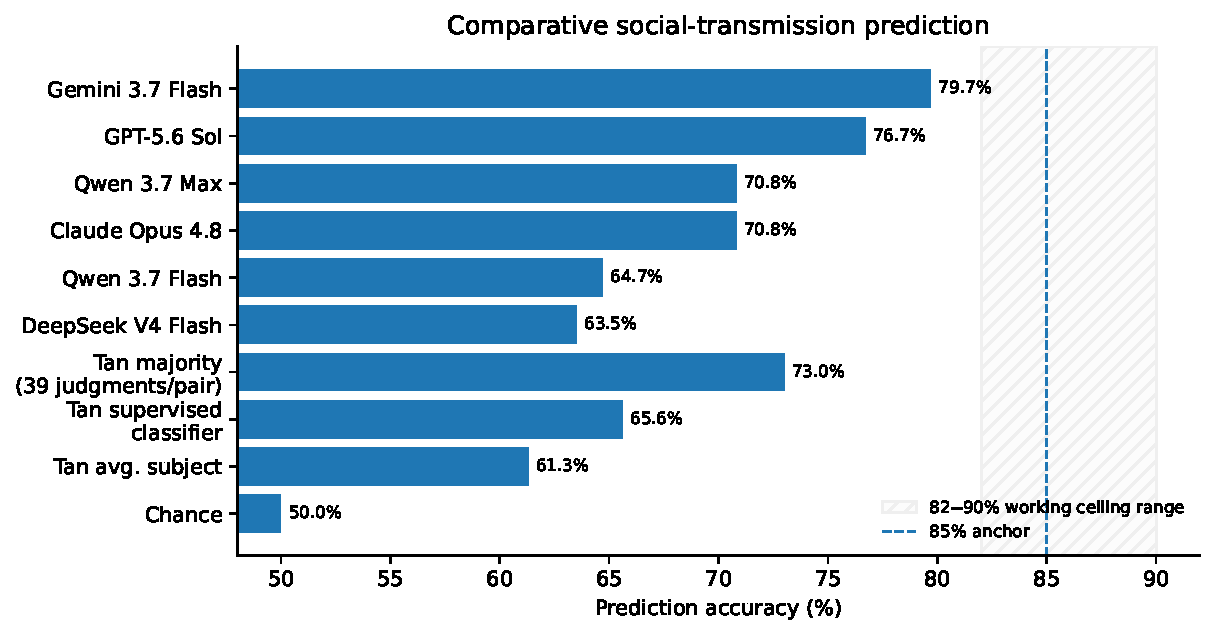
\includegraphics[width=.88\linewidth]{figures/chi_fig_benchmark_revised.pdf}
\caption{Historical comparative social-transmission prediction. Current model bars use 1,142 HypoBench pairs. Tan et al.'s human references are 61.3\% average-subject and 73.0\% majority-vote accuracy over 39 judgments per pair; their held-out supervised classifier reached 65.6\%. The shaded 82--90\% region is the sensitivity envelope around the 85\% practical text-only ceiling.}
\Description{Horizontal chart showing current model accuracies from 63.5 to 79.7 percent, historical human and supervised references, and an 82 to 90 percent practical text-only ceiling region.}
\label{fig:benchmark}
\end{figure*}

\begin{table}[t]
\caption{Frozen historical benchmark. Human rows are historical references; model CIs are Wilson intervals over 1,142 pairs.}
\label{tab:benchmark}
\centering\small
\setlength{\tabcolsep}{1.6pt}
\begin{tabular}{@{}lrrr@{}}
\toprule
Predictor & Acc. & $S_{85}$ & 95\% CI \\
\midrule
Gemini 3.7 Flash & 79.7\% & .85 & 77.3--81.9 \\
GPT-5.6 Sol & 76.7\% & .76 & 74.2--79.1 \\
Qwen 3.7 Max & 70.8\% & .59 & 68.0--73.3 \\
Claude Opus 4.8 & 70.8\% & .59 & 68.1--73.4 \\
Qwen 3.7 Flash & 64.7\% & .42 & 61.9--67.4 \\
DeepSeek V4 Flash & 63.5\% & .39 & 60.7--66.2 \\
\midrule
Tan avg. subject & 61.3\% & .32 & -- \\
Tan majority (39 judgments/pair) & 73.0\% & .66 & -- \\
Tan supervised classifier & 65.6\% & .45 & -- \\
\bottomrule
\end{tabular}
\end{table}

\begin{figure}[t]
\centering
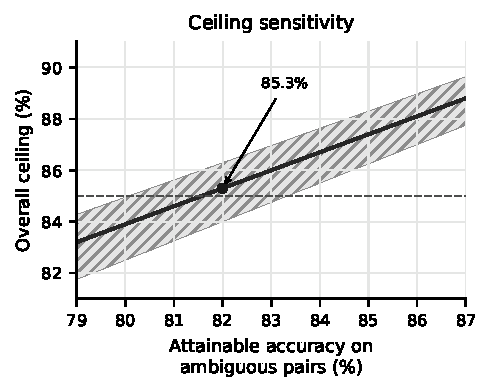
\includegraphics[width=\linewidth]{figures/chi_fig_ceiling.pdf}
\caption{Sensitivity of the practical text-only ceiling. The central assumptions give 85.3\%; the envelope spans approximately 82--90\%.}
\Description{Sensitivity plot centered near an 85.3 percent practical text-only ceiling with an approximately 82 to 90 percent envelope.}
\label{fig:ceiling}
\end{figure}

\subsection{RQ2: LLMs outperform contemporary humans on identical narratives}
Round-1 human sessions averaged 10.86/20 correct, or 54.3\%. The game's featured robot won 69 of 70 completed rounds. More importantly, every fixed model family exceeds the matched recorded human choices in aggregate.

Table~\ref{tab:matched} shows the fixed comparisons. Gemini is 77.7\% correct versus 54.1\% for the same 1,380 judgments, a +23.6-point gap; the crossed session/item bootstrap interval is +17.6 to +29.4 points. GPT-5.6 Sol reaches a +22.0-point gap. Even DeepSeek, the weakest model in the panel, remains +8.2 points ahead with a +1.9 to +14.5 interval. At the frontier, the +23.6-point advantage corresponds to about 4.7 additional correct choices per 20-item round.

\begin{table*}[t]
\caption{Matched Round-1 fixed-model comparisons. Gap intervals use a 20,000-resample crossed session/item bootstrap. ``H/T/M wins'' compares 20-item human/model scores on complete-coverage sessions.}
\label{tab:matched}
\centering\small
\begin{tabular}{lrrrrrrr}
\toprule
Model & Sessions & Human acc. & Model acc. & Gap & 95\% gap interval & H/T/M wins \\
\midrule
Gemini 3.7 Flash & 69 & 54.1\% & 77.7\% & +23.6 pp & +17.6,+29.4 & 1/0/68 \\
GPT-5.6 Sol & 69 & 54.1\% & 76.1\% & +22.0 pp & +16.2,+27.6 & 2/2/65 \\
Qwen 3.7 Max & 62 & 54.2\% & 70.5\% & +16.3 pp & +9.9,+22.6 & 4/3/55 \\
Claude Opus 4.8 & 69 & 54.1\% & 68.9\% & +14.8 pp & +8.7,+20.8 & 5/7/57 \\
Qwen 3.7 Flash & 69 & 54.1\% & 64.7\% & +10.6 pp & +4.7,+16.4 & 10/7/52 \\
DeepSeek V4 Flash & 69 & 54.1\% & 62.3\% & +8.2 pp & +1.9,+14.5 & 16/7/46 \\
\bottomrule
\end{tabular}
\end{table*}

The sole featured-robot winner scored 16/20 and beat all six models on that set. Removing that session lowers overall human accuracy only from 54.3 to 53.9\%, so the aggregate comparison does not depend on the top human score.

\subsection{Human--model disagreements expose complementary predictive signal}
Human and model choices disagree on roughly 39--44\% of matched trials. On those disagreements, Gemini is correct on 77.7\% of 587 cases, GPT-5.6 Sol on 76.4\%, and DeepSeek on 59.4\%, with the other models in between. The model advantage therefore remains concentrated precisely where the human and model choose different alternatives.

\begin{figure*}[t]
\centering
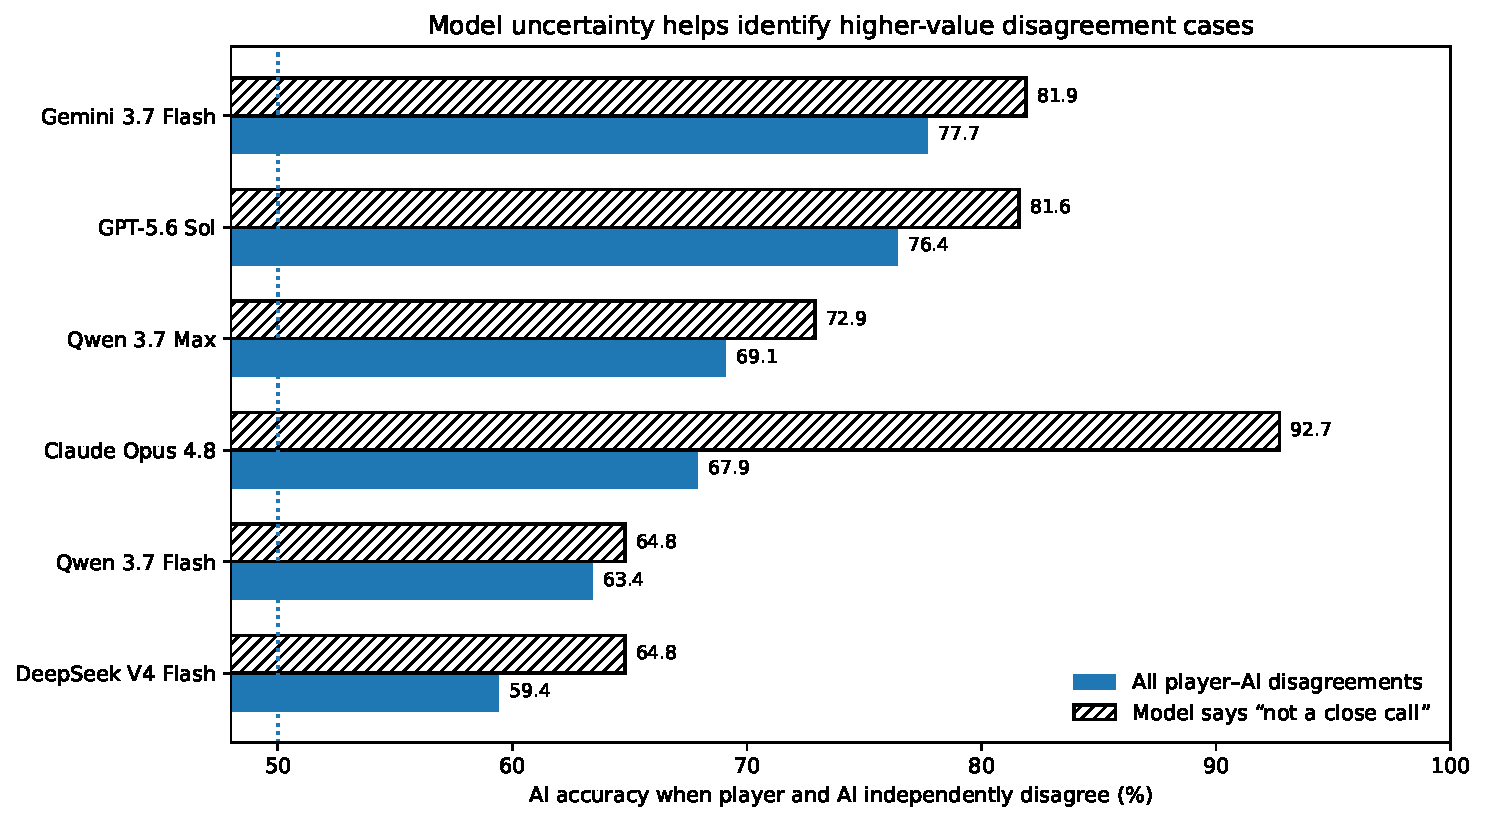
\includegraphics[width=.86\linewidth]{figures/chi_fig_disagreement.pdf}
\caption{Model accuracy conditional on independent human--model disagreement in the public-game records. Hatched bars retain only disagreements the model labels non-close.}
\Description{Grouped bars showing model accuracy on all human-model disagreements and on the subset the model labels non-close.}
\label{fig:disagreement}
\end{figure*}

\subsection{RQ3: model uncertainty supports selective prediction}
The frozen 1,142-pair close-call field is informative for every model. Gemini is 84.7\% correct on 835 predictions it labels non-close versus 66.1\% on 307 close calls; GPT-5.6 Sol is 79.8\% versus 62.2\%, and Claude is 90.5\% versus 64.3\%. The same pattern appears inside human--model disagreements, where non-close predictions are substantially more accurate for the strongest models.

The explicit 100-pair confidence experiment strengthens this result. Table~\ref{tab:confidence} reports accuracy, Brier score, ECE, and selective accuracy. The most-confident quartile reaches 92\% for Gemini and 96\% for both GPT-5.6 Sol and Claude; top-half accuracy is 88--90\%. Confidence therefore provides a strong ranking signal for selective use.

\begin{table}[t]
\caption{Explicit confidence on the deterministic 100-pair robustness sample. ECE uses five bins.}
\label{tab:confidence}
\centering\small
\setlength{\tabcolsep}{2.1pt}
\begin{tabular}{@{}lrrrrr@{}}
\toprule
Model & Acc. & Mean conf. & Brier & ECE & Top 25\% \\
\midrule
Gemini 3.7 Flash & 80\% & 74.1\% & .151 & .099 & 92\% \\
GPT-5.6 Sol & 77\% & 72.6\% & .162 & .061 & 96\% \\
Claude Opus 4.8 & 74\% & 67.8\% & .180 & .086 & 96\% \\
\bottomrule
\end{tabular}
\end{table}

\subsection{RQ4: the frontier survives prompt and order perturbations}
Across the paper prompt and a concise equivalent rephrasing, Gemini varies from 79 to 82\%, GPT from 73 to 80\%, and Claude from 74 to 75\%. Canonical predictions agree across the two prompt wordings on 83--93\% of pairs.

Reversing X/Y order yields canonical-choice consistency of 90\% for Gemini, 88\% for GPT, and 80\% for Claude. Swapped-order accuracy is 83\%, 79\%, and 73\% respectively. Thus neither equivalent prompt wording nor label order removes the high-accuracy regime.

\begin{table*}[t]
\caption{Prompt and orientation robustness on 100 deterministic historical pairs. Prompt range is max--min accuracy across two equivalent prompts; prompt agreement is identical canonical choice across them.}
\label{tab:robustness}
\centering\small
\begin{tabular}{lrrrrrr}
\toprule
Model & Prompt acc. range & Prompt agreement & Order consistency & Original acc. & Swapped acc. & $\Delta$ \\
\midrule
Gemini 3.7 Flash & 79--82\% & 93\% & 90\% & 79\% & 83\% & +4 pp \\
GPT-5.6 Sol & 73--80\% & 83\% & 88\% & 73\% & 79\% & +6 pp \\
Claude Opus 4.8 & 74--75\% & 87\% & 80\% & 75\% & 73\% & -2 pp \\
\bottomrule
\end{tabular}
\end{table*}

\subsection{RQ5: fresh Bluesky outcomes reproduce the signal}
On 48 fresh high-signal Bluesky pairs, Gemini predicts 36 correctly: 75.0\% (95\% Wilson CI 61.2--85.1). Among complete runs, the five-current-model panel averages 65.8\% versus 55.2\% for four older models, a +10.6-point case-paired difference. The exact two-sided sign-flip test over 48 case-level panel differences gives $p=.030$; a 100,000-resample paired bootstrap gives a 95\% interval of +1.4 to +19.6 points.

These newly collected outcomes extend the comparative signal beyond the old Twitter/HypoBench label set and show a clear current-versus-older panel separation on the frozen fresh sample.

\begin{figure}[t]
\centering
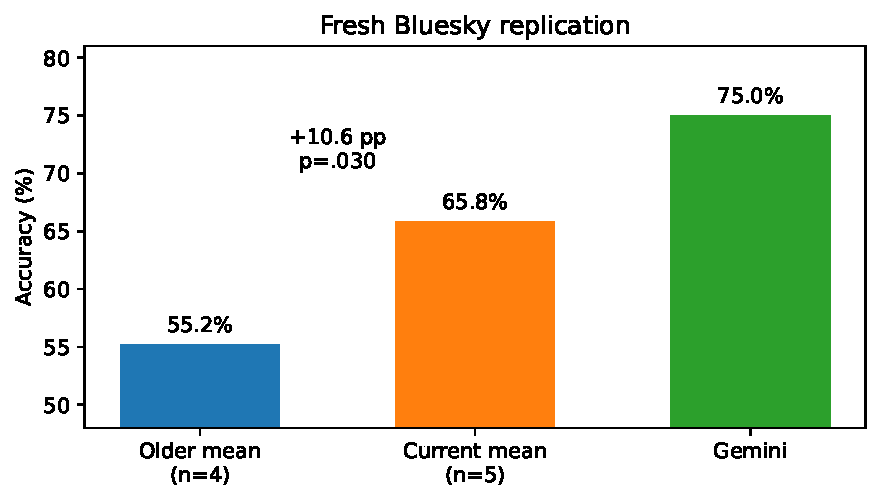
\includegraphics[width=\linewidth]{figures/chi_fig_bluesky.pdf}
\caption{Fresh August 2026 Bluesky replication on 48 high-signal same-author/same-destination pairs. Five complete current-model runs average 65.8\%, four older-model runs 55.2\%, and Gemini reaches 75.0\%.}
\Description{Bars showing 55.2 percent for the older-model panel, 65.8 percent for the complete current-model panel, and 75.0 percent for Gemini.}
\label{fig:bluesky}
\end{figure}

\section{What the Results Reveal About LLMs and Human Judgment}
\subsection{The models appear to know more about audience preference than their prose suggests}
The central comparison is between \emph{judges}, not writers. Humans and LLMs see the same human-authored alternatives and predict which narrative an audience chose to retransmit. Across both the historical references and the direct contemporary comparison, the strongest LLMs recover substantially more of that behavioral signal; Gemini reaches 77.7\% where matched recorded human choices reach 54.1\%.

That matters beyond retweet prediction. Social transmission is one observable consequence of narrative quality: people do not merely register approval but choose to carry a message into their own social context. Fresh Bluesky outcomes and prompt/order perturbations point to the same capability from different directions. The strongest models therefore appear to encode audience-preference information that is considerably richer than the generic quality of their default generations would suggest.

\subsection{Confidence and generation implications}
Model judgments are not equally reliable. Close-call and explicit-confidence signals identify much stronger subsets, reaching 92--96\% in the most-confident quartile of the 100-pair diagnostic. This supports selective evaluation: use the audience model most strongly where its confidence has empirical value.

The result also separates evaluation from generation. A model can recognize which human-written narrative is more likely to spread even when its own prose is mediocre. That makes evaluation-guided generation a concrete systems hypothesis: generate alternatives, score them with an audience-response evaluator, then select or revise. The practical opportunity is to make generation use preference knowledge that appears already to be present in the model.

\section{Limitations and Scope}
The claim is task-specific: comparative prediction of \emph{aggregate social transmission} between matched human-authored alternatives. Retransmission is a consequential revealed-preference signal, but it is not identical to liking, aesthetic quality, or individual preference: people also share for identity, information, social utility, disagreement, or other communication motives. The result is therefore evidence about which narratives audiences choose to propagate, not a universal ranking of prose quality. It is not universal human superiority, personal-preference prediction, or a causal estimate of why one message spread more. The Twitter pairs are observational; author and destination are controlled, while time, exposure, media, and cascade state are not.

Tan et al.'s human numbers are cross-study baselines from a separate 100-pair experiment. The direct paired evidence comes from the contemporary web study, which is a convenience sample of sessions: 69 of 70 completions self-report non-native English, identity is unverified, repeat participation cannot be excluded, and 99 starts yielded 70 Round-1 completions. Later rounds had only eight and two completions. The crossed bootstrap clusters sessions and items, not latent unique people.

The 85\% ceiling is a model-based estimate, not an identified constant. Its conceptual basis is residual outcome information outside the text; its numerical basis is the two-regime sensitivity model anchored to Tan et al.'s consensus structure. The reported 82--90\% envelope shows sensitivity, and predictors with timing, network, media, or early-cascade information solve a richer problem that may exceed this text-only ceiling.

The robustness experiment covers three models and 100 pairs. X/Y reversal changes 10--20\% of canonical choices, so positional sensitivity remains. Confidence metrics are also based on $n=100$ per model. Historical Wilson intervals are pair-level binomial intervals and do not model clustering by recurring author or destination.

Human--model disagreement is not an intervention study: players did not receive model advice on primary trials. Likewise, ranking external human-written alternatives does not establish that a model can generate the better alternative on demand or self-evaluate reliably during generation.

The Bluesky replication is small ($n=48$), high-signal, manually audited, observational, and drawn from a replay that hit a byte quota. Panel inference uses five complete current and four older runs; DeepSeek produced 28/48 valid outputs. The fresh result shows that the capability extends beyond the historical label set but cannot prove that every Twitter item was absent from training. Hosted endpoints can also change, so frozen outputs and manifests are the authoritative reproduction target.

\section{Future Work: From Evaluation to Generation}
The next experiment is intervention: generate several alternatives under a fixed compute budget, rank them with an independently prompted audience evaluator, and compare the selected output with equal-compute generation baselines. The confidence results also motivate selective evaluation, allocating extra search or revision only when the evaluator is sufficiently confident.

A second direction is live self-evaluation. Humans can overvalue their own work (the ``IKEA effect''; \citealp{norton2012}); LLMs may show a similar bias. Comparing live, post-generation, and blind-replay scores would test whether audience judgment survives generation.

\section{Transparency and Reproducibility}
The public repository at \url{https://github.com/victorlavrenko/llms-read-the-room} contains deidentified Round-1 trial/session data and protocol material; model aggregate, disagreement, close-call, and calibration analyses; the frozen 48-pair Bluesky data, collection/finalization code, manifests, raw/scored outputs, and analysis; the historical benchmark summary and pinned pair-level snapshot; the ceiling script; and the exact 100-pair robustness protocol with raw OpenRouter responses, prompt/order/confidence outputs, CSV analyses, and the crossed session/item bootstrap used for Table~\ref{tab:matched}. Model IDs, temperature, token limits, retry policy, seeds, parsing rules, and dataset hashes are preserved.

\section{Conclusion}
The central result is a paradox: models that are often criticized for generic ``AI slop'' can nevertheless predict which human-written narratives people will retransmit substantially better than the human judges available here. Gemini reaches 79.7\% on 1,142 historical same-author/same-destination Twitter pairs and 77.7\% versus 54.1\% for matched contemporary human choices, a +23.6-point gap. All six fixed model families show positive matched gaps. Prompt/order perturbations preserve the frontier result, confidence isolates 92--96\% top-quartile subsets, and fresh Bluesky outcomes reproduce the signal beyond the historical label set.

A practical 85\% text-only ceiling places the frontier near the upper range expected from text alone: across the 82--90\% sensitivity envelope, the strongest model captures roughly 74--93\% of the modeled improvement from chance to the ceiling. The broader implication is that generation and preference knowledge are separable. Current LLMs may already know much more about what human audiences appreciate than their default prose reveals. The next systems question is how to make generation exploit that knowledge: generate, compare, select, and revise.

\section*{AI Assistance Disclosure}
ChatGPT (OpenAI) was used for language editing, structural revision, literature-check assistance, code generation for robustness/statistical analyses, and consistency checking. The author selected the research questions and methods, ran or supervised the experiments, inspected the frozen artifacts and generated analyses, made the substantive interpretation decisions, and takes responsibility for the paper and its claims.

{\clubpenalty=10000\widowpenalty=10000
\begin{thebibliography}{99}
\scriptsize
\setlength{\itemsep}{0pt}
\setlength{\parskip}{0pt}
\bibitem[Berger and Milkman(2012)]{berger2012}
Jonah Berger and Katherine L. Milkman. 2012. What Makes Online Content Viral? \emph{Journal of Marketing Research} 49, 2 (2012), 192--205. \url{https://doi.org/10.1509/jmr.10.0353}.

\bibitem[Berger(2025)]{berger2025}
Jonah Berger. 2025. What Gets Shared, and Why? Interpersonal Communication and Word of Mouth. \emph{Annual Review of Psychology} 76 (2025), 559--581.

\bibitem[Boji\'{c} et~al.(2026)]{bojic2026}
Ljubi\v{s}a Boji\'c, Alexander Felfernig, Bojana Dini\'c, Velibor Ili\'c, Achim Rettinger, Vera Mevorah, Damian Trilling, et al. 2026. Persona-prompted LLM agents achieve modest but genuine prediction of human social media reactions. \emph{Scientific Reports} 16 (2026), 27684. \url{https://doi.org/10.1038/s41598-026-66277-8}.

\bibitem[El-amrany et~al.(2025)]{elamrany2025}
Samir El-amrany, Matthias R. Brust, Salima Lamsiyah, and Pascal Bouvry. 2025. Reddit-V: A Virality Prediction Dataset and Zero-Shot Evaluation with Large Language Models. In \emph{Proceedings of RANLP 2025}. 334--341.

\bibitem[Huang et~al.(2024)]{huang2024}
Jie Huang, Xinyun Chen, Swaroop Mishra, Huaixiu Steven Zheng, Adams Wei Yu, Xinying Song, and Denny Zhou. 2024. Large Language Models Cannot Self-Correct Reasoning Yet. In \emph{International Conference on Learning Representations (ICLR 2024)}. \url{https://arxiv.org/abs/2310.01798}.

\bibitem[Kadavath et~al.(2022)]{kadavath2022}
Saurav Kadavath et al. 2022. Language Models (Mostly) Know What They Know. \emph{arXiv preprint arXiv:2207.05221}. \url{https://arxiv.org/abs/2207.05221}.

\bibitem[Liu et~al.(2025)]{liu2025hypo}
H. Liu, S. Huang, J. Hu, Y. Zhou, and C. Tan. 2025. HypoBench: Towards Systematic and Principled Benchmarking for Hypothesis Generation. arXiv:2504.11524.

\bibitem[Madaan et~al.(2023)]{madaan2023}
Aman Madaan, Niket Tandon, Prakhar Gupta, Skyler Hallinan, Luyu Gao, Sarah Wiegreffe, Uri Alon, et al. 2023. Self-Refine: Iterative Refinement with Self-Feedback. In \emph{Advances in Neural Information Processing Systems 36 (NeurIPS 2023)}. \url{https://arxiv.org/abs/2303.17651}.

\bibitem[Norton et~al.(2012)]{norton2012}
Michael I. Norton, Daniel Mochon, and Dan Ariely. 2012. The IKEA Effect: When Labor Leads to Love. \emph{Journal of Consumer Psychology} 22, 3 (2012), 453--460. \url{https://doi.org/10.1016/j.jcps.2011.08.002}.

\bibitem[Tan et~al.(2014)]{tan2014}
Chenhao Tan, Lillian Lee, and Bo Pang. 2014. The Effect of Wording on Message Propagation: Topic- and Author-Controlled Natural Experiments on Twitter. In \emph{Proceedings of ACL 2014}. Association for Computational Linguistics, 175--185. \url{https://doi.org/10.3115/v1/P14-1017}.

\bibitem[Yuan et~al.(2024)]{yuan2024}
Weizhe Yuan, Richard Yuanzhe Pang, Kyunghyun Cho, Xian Li, Sainbayar Sukhbaatar, Jing Xu, and Jason E. Weston. 2024. Self-Rewarding Language Models. In \emph{Proceedings of the 41st International Conference on Machine Learning}, PMLR 235, 57905--57923. \url{https://proceedings.mlr.press/v235/yuan24d.html}.
\end{thebibliography}
}
\end{document}
